%---------------------------------------------------------------------------%
%-                                                                         -%
%-                          Beamer Template                                -%
%-                                                                         -%
%---------------------------------------------------------------------------%
%- Copyright (C) Huangrui Mo <huangrui.mo@gmail.com> 
%- This is free software: you can redistribute it and/or modify it
%- under the terms of the GNU General Public License as published by
%- the Free Software Foundation, either version 3 of the License, or
%- (at your option) any later version.
%---------------------------------------------------------------------------%
%->> Document class declaration
%---------------------------------------------------------------------------%
\documentclass[compress,table,aspectratio=169,xcolor={usenames,dvipsnames}]{beamer}%

%---------------------------------------------------------------------------%
%->> Document settings
%---------------------------------------------------------------------------%
\usepackage[biber,authoryear,tikz,table]{Style/artrabeamer}% document settings

\usepackage{Style/artracom}% user defined commands
%---------------------------------------------------------------------------%
%->> Document inclusion
%---------------------------------------------------------------------------%
%\includeonly{Tex/Sec_Introduction}% selected files compilation
%\includeonlylecture{lecture label}% selected lectures compilation
%---------------------------------------------------------------------------%
%->> Theme settings
%---------------------------------------------------------------------------%
%-
%-> Recommended theme combinations
%-
%- set: [<usetheme>, <useoutertheme>, <useinnertheme>, <usecolortheme>]
%- light: [<CambridgeUS>, <miniframes>, <circle>, <dove|seahorse|beaver|seagull>]
%- light: [<Boadilla|Madrid>, <default>, <circle>, <dove|seahorse|beaver|seagull>]
%- dark: [<Boadilla|Madrid>, <default>, <circle>, <fly|albatross>]
%-
%-> Global themes
%-
\usetheme{CambridgeUS}%
%- Options:
%- [<Boadilla|CambridgeUS|default|...>]
%- It is the complete theme in the sense that they control just about every aspect
%- of a slide's appearance. Think of it as major theme.
%- Theme Matrix (https://www.hartwork.org/beamer-theme-matrix/) contains the
%- various theme and color combinations included with beamer.
%-
%-> Outer themes
%-
%\useoutertheme{}%
%- Options:
%- [<default|infolines|miniframes|smoothbars|sidebar|split|shadow|tree|smoothtree>]
%- An outer theme dictates (roughly) the overall layout of frames. It specifies where
%- any navigational elements should go (like a mini table of contents or navigational
%- mini frames) and what they should look like. Typically, an outer theme specifies
%- how the following elements are rendered:
%- - The headline and footline.
%- - The sidebars.
%- - The logo.
%- - The frame title.
%- The Beamer User Guide explains each theme with examples.
%-
%- *** Miniframes
\useoutertheme[%
    %footline=empty,% suppressed the footline (default).
    %footline=authorinstitute,% shows the author's name and the institute in the footline.
    %footline=authortitle,% shows the author's name and the title in the footline.
    %footline=institutetitle,% shows the institute and the title in the footline.
    %footline=authorinstitutetitle,% shows all three in the footline.
    subsection=false,% shows or suppresses line showing the subsection in the headline.
]{miniframes}%
%-
%- *** Sidebar
%\useoutertheme[%
%    %left,% sidebar links.
%    %right,% sidebar rechts.
%    %hideallsubsections,% suppresses all subsections.
%    %hideothersubsections,% suppresses all subsections except the current one.
%]{sidebar}%
%-
%-> Inner themes
%-
\useinnertheme{circles}
\setbeamertemplate{navigation symbols}{}

\usecolortheme{dove}%
%%---------------------------------------------------------------------------%
%->> Configuration
%---------------------------------------------------------------------------%
%-> Titlepage information
%-

%---------------------------------------------------------------------------%
%->> Document inclusion
%---------------------------------------------------------------------------%
%\includeonly{Tex/Sec_Introduction,Tex/Sec_Method,Tex/Sec_Result,Tex/Sec_Conclusion}% selected files compilation
%\includeonlylecture{lec_present_intro,lec_present_method,lec_present_result,lec_present_conclude}% selected lectures compilation
%\includeonlyframes{fra_current}% selected frames compilation
%---------------------------------------------------------------------------%
%->> Titlepage information
%---------------------------------------------------------------------------%
\title[]% optional, abbreviated title
{\enorcn{Beamer Report}{Beamer 报告}}

\subtitle% optional
{-- \enorcn{A Beamer template for easily positioning and manipulating content}{可轻松安置和操纵内容的Beamer模板}}

\author[]% optional, abbreviated authors
{\enorcn{Huangrui Mo}{\large莫晃锐}}

\institute[]% optional, abbreviated name
{
  %\inst{*}%
  %\enorcn{Mechanical and Mechatronics Engineering, University of Waterloo}{\small 加拿大滑铁卢大学}
  %\and
  %\inst{\dag}%
  %\enorcn{Center for Combustion Energy, Tsinghua University}{\small 清华大学燃烧能源中心}
  %\and
  %\inst{+}%
  \enorcn{Institute of Mechanics, CAS}{中国科学院力学研究所}
}

\date[]{\enorcn{October 28, 2021}{2021年10月28日}}% or simply: \date{\today}
%\date[IDS 2018]{International Detonation Symposium, 2018}% conference name

\subject{\enorcn{Report by Huangrui Mo}{莫晃锐报告}}% inserted into the PDF information catalog

%\logo{\tikzart[t=p,x=8,y=-6,w=4]{logo_uw}}% on each slide 
\titlegraphic{\tikzart[t=p,x=0,y=-4,w=4]{logo_uw}}% only on title page
% can also use any field given by \author, \title, \date, \institute, or \tikz to place image in the title page
%\addtobeamertemplate{headline}{}{% on each slide with headline
%    \tikzart[t=p,x=8,y=7,w=4]{logo_uw}
%}
%---------------------------------------------------------------------------%
%
\begin{document}

%---------------------------------------------------------------------------%
%->> Frontmatter
%---------------------------------------------------------------------------%
%---------------------------------------------------------------------------%
%->> Create titlepage
%---------------------------------------------------------------------------%
%- create the title page, \frame[plain]{\titlepage} for a titlepage filling the whole frame.
{% these braces make the change local to the single frame.
    \setbeamertemplate{headline}{%
        \begin{beamercolorbox}[wd=\paperwidth,ht=2.5ex,dp=1.5ex,right]{section in head/foot}%
        \end{beamercolorbox}%
    }
    \setbeamertemplate{footline}{%
        \leavevmode%
        \hbox{%
            \begin{beamercolorbox}[wd=.333333\paperwidth,ht=2.25ex,dp=1ex,center]{author in head/foot}%
            \end{beamercolorbox}%
            \begin{beamercolorbox}[wd=.333333\paperwidth,ht=2.25ex,dp=1ex,center]{title in head/foot}%
            \end{beamercolorbox}%
            \begin{beamercolorbox}[wd=.333333\paperwidth,ht=2.25ex,dp=1ex,right]{date in head/foot}%
            \end{beamercolorbox}}%
        \vskip0pt%
    }
    \begin{frame}[plain]
        \titlepage%
        %\tikzart[t=p,x=0,y=-4,w=4]{logo_uw}
        \addtocounter{framenumber}{-1}% modify the counter to exclude a frame from total count
    \end{frame}%
}
%---------------------------------------------------------------------------%
%->> Outline page
%---------------------------------------------------------------------------%
%\section[Outline]{}%
%\begin{frame}[plain]%
%    \frametitle{Outline}%
%    \tableofcontents%[part=partid]% may add the option [pausesections]
%    \addtocounter{framenumber}{-1}% modify the counter to exclude a frame from total count
%\end{frame}%
\AtBeginPart% [<Lecture|Part|Section>]% insert content at the beginning of each element
{%
    \frame[plain]{\partpage}% [<partpage|sectionpage>][<\insertlecture|\insertpart|\insertsection>]
    %\begin{frame}[plain]%
    %    \frametitle{Outline}%
    %    {%
    %        \tableofcontents[sectionstyle=show/show,subsectionstyle=show/show/show]%
    %    }%
    %\end{frame}%
}
%---------------------------------------------------------------------------%
%->> Content centering
%---------------------------------------------------------------------------%
%\centering% automatic horizontal centering of frame content
%---------------------------------------------------------------------------%


\begin{frame}[fragile]

	\begin{figure}
		\centering
		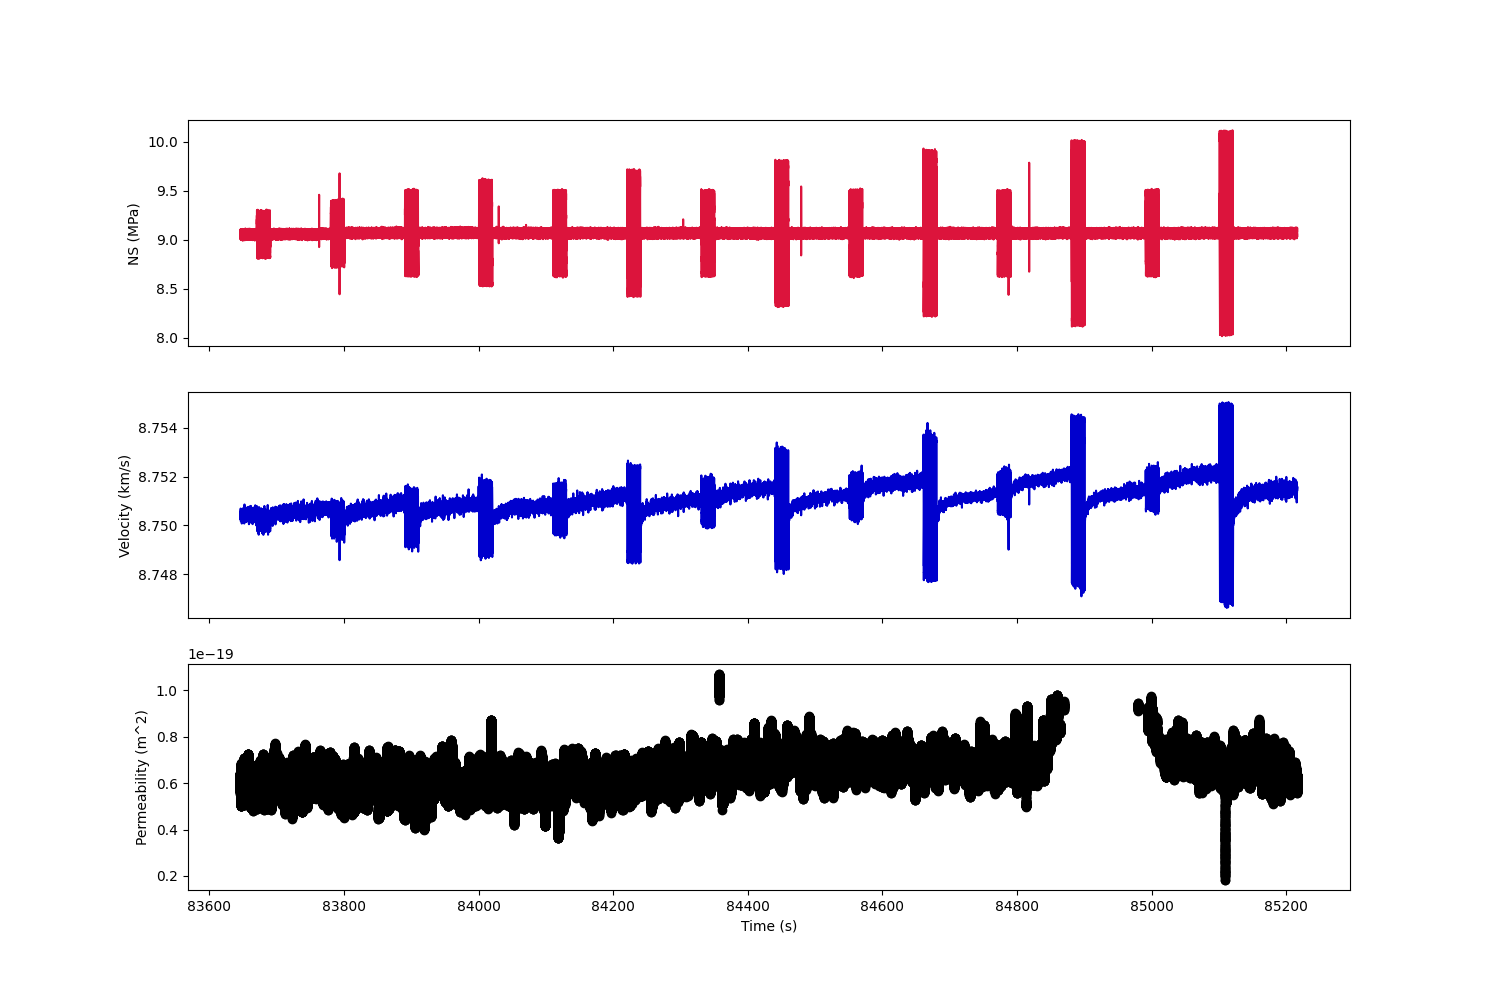
\includegraphics[height=8cm]{../rel_chg_analysis/p5607_run1_prelim_tr5.png}
	\end{figure}

\end{frame}

\begin{frame}[fragile]{}

	\begin{figure}
		\centering
		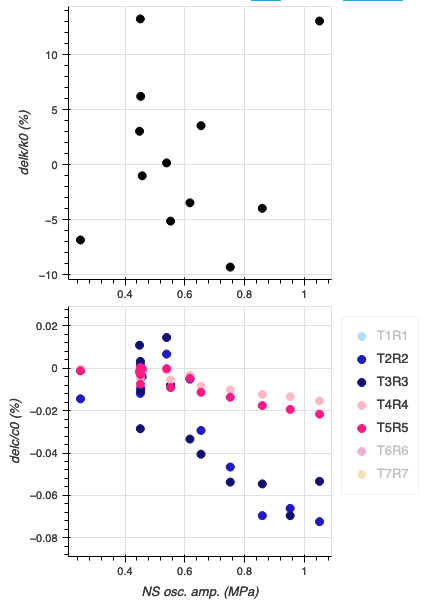
\includegraphics[height=6cm]{../rel_chg_analysis/p5607_run1_prelim_delc_NS.png}
	\end{figure}

\end{frame}
%

\begin{frame}[fragile]{}
	
	\begin{alertblock}{To-do:}
		\begin{itemize}
			\item fix x-corr windows for following pairs: TR1, TR6, TR7
			\item update velocity function with new sideblock geometry
		\end{itemize}
	\end{alertblock}
	

\end{frame}


\end{document}
%---------------------------------------------------------------------------%
